\documentclass{article}

\usepackage{amssymb}
\usepackage[utf8]{inputenc}
\usepackage{graphicx}
\usepackage[section]{placeins}
\usepackage[
bookmarks=true,
colorlinks=true,
breaklinks=true,
urlcolor=red,
citecolor=blue,
linkcolor=black,
unicode=true,
]
{hyperref}

\begin{document}
\section{Lineární klasifikátory, Perceptronový algoritmus}
Bayesovské rozhodování používalo ztrátovou funkci, apriorní a aposteriorní pravděpodobnosti, nebayesovské si vystačilo s aposteriorními pravděpodobnostmi. Lineární klasifikátory nepotřebují ani to. Jejich klasifikace je založena pouze na dodané trénovací množině $T = \{(x_1, k_1), ..., (x_l, k_l)\}$. Výhody a nevýhody tohoto přístupu v Figure \ref{fig:pros_cons}.

\begin{figure}[h]
\begin{center}
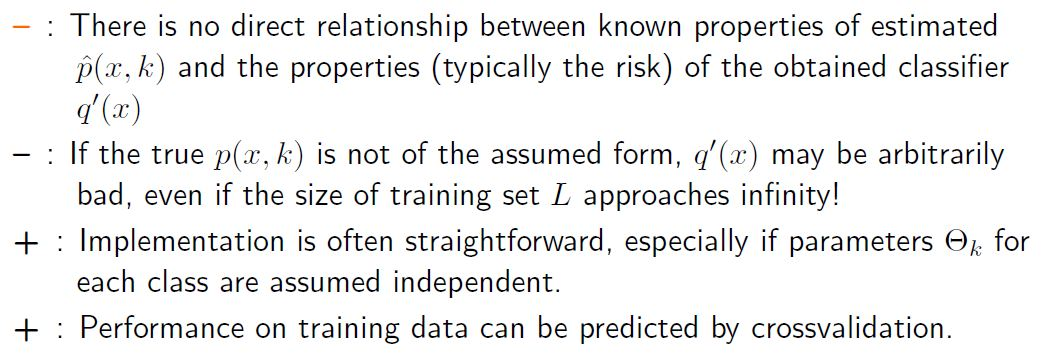
\includegraphics[width=12cm]{pros_cons.jpg}
\caption{Výhody a nevýhody lin. klasifikátorů}
\label{fig:pros_cons}
\end{center}
\end{figure} 

\subsection{Perceptron learning}

Algorimus očekává na vstupu trénovací množinu pozorování $T = \{x'_1, ..., x'_l\}$ kde $x'_j = k_j \cdot [x_j\ 1]$ (tzn. množina souřadnic pozorování kde ke každému pozorování přidáme 1 a vynásobíme klasifikací $k_j \in \{-1, 1\}$). Výstup algoritmu je vektor vah $w' = [w\ b]$ takových, že $\langle w', x'_j \rangle \geq 0, \forall j \in \{1,...,l\}$. Vlastní algoritmus je popsán ve Figure \ref{fig:perceptron}. 

\begin{figure}[h]
\begin{center}
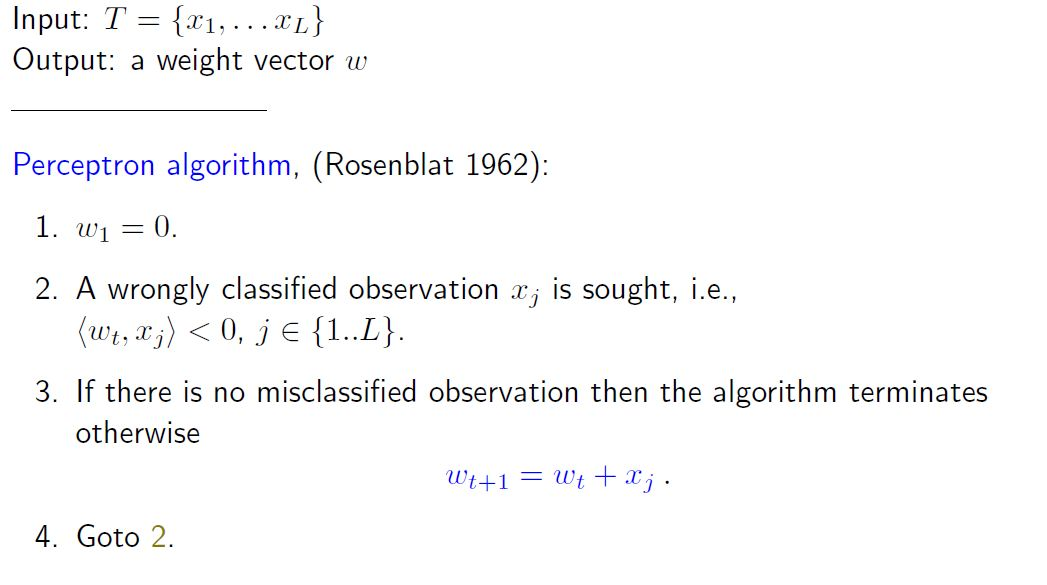
\includegraphics[width=12cm]{perceptron.jpg}
\caption{Perceptron popis}
\label{fig:perceptron}
\end{center}
\end{figure} 

\subsubsection{Neseparovatelná data}

Modifikace algoritmu popsána ve Figure \ref{fig:nonsepperceptron}. 

\begin{figure}[h]
\begin{center}
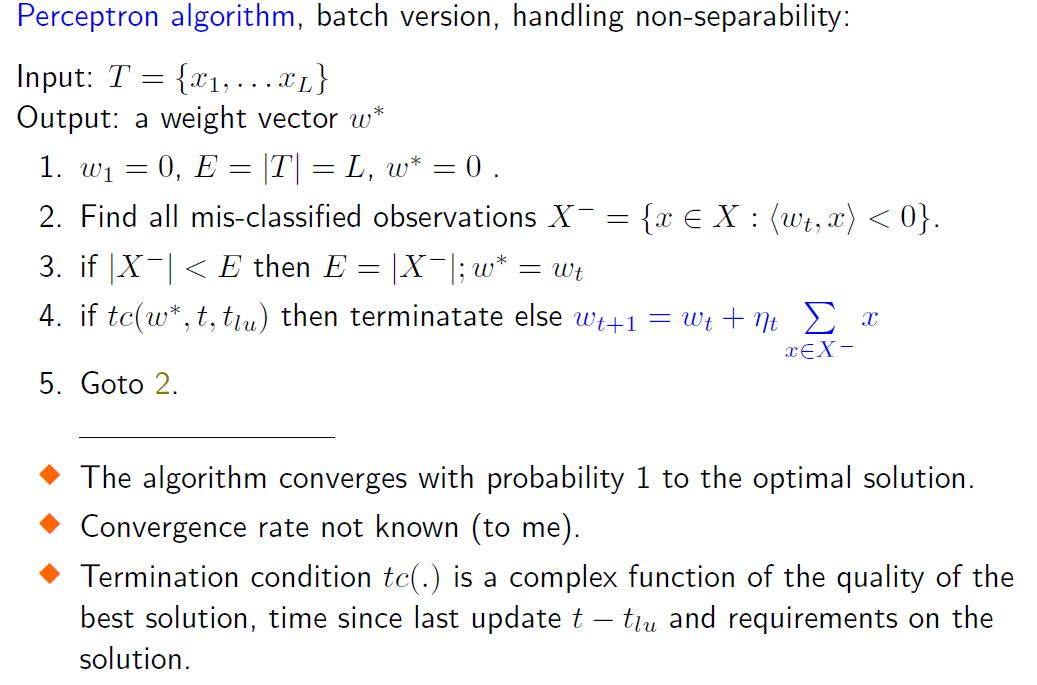
\includegraphics[width=12cm]{nonseparable_perceptron.jpg}
\caption{Perceptron popis s neseparovatelnými daty}
\label{fig:nonsepperceptron}
\end{center}
\end{figure} 
\end{document}